\documentclass[border=4pt]{standalone}
\usepackage{tikz}
\usepackage{amsmath,amssymb}
\usepackage{mathptmx}
\usetikzlibrary{arrows.meta,positioning,calc,shapes.geometric,decorations.pathreplacing,shadows,fadings,patterns}
\definecolor{cblue}{HTML}{1F4E9C}
\definecolor{cgold}{HTML}{D08C00}
\definecolor{cred}{HTML}{B5172E}
\definecolor{cgreen}{HTML}{1B7A3A}
\definecolor{cgrey}{HTML}{555555}
\definecolor{cpurple}{HTML}{5B2A86}
% oblique 3D cuboid: \cuboid{x}{y}{z}{dx}{dy}{dz}{colour}
\newcommand{\cuboid}[7]{%
  \fill[#7!55!white,draw=#7!60!black,line width=0.4pt] (#1,#2,#3+#6) -- ++(#4,0,0) -- ++(0,#5,0) -- ++(-#4,0,0) -- cycle;
  \fill[#7!80!black,draw=#7!60!black,line width=0.4pt] (#1+#4,#2,#3) -- ++(0,#5,0) -- ++(0,0,#6) -- ++(0,-#5,0) -- cycle;
  \fill[#7,draw=#7!60!black,line width=0.4pt] (#1,#2,#3) -- ++(#4,0,0) -- ++(0,0,#6) -- ++(-#4,0,0) -- cycle;}

\begin{document}
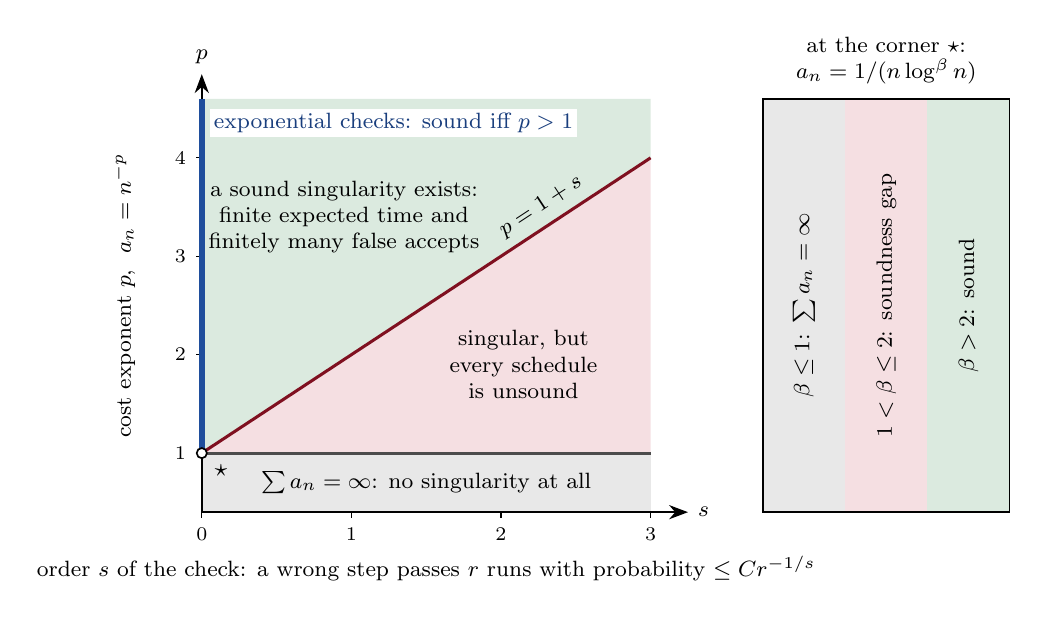
\begin{tikzpicture}[x=1.9cm,y=1.25cm,lab/.style={font=\footnotesize,align=center}]
% regions: s in [0,3], p in [0.4,4.6]
\fill[gray!18] (0,0.4) rectangle (3,1);
\fill[cred!14] (0,1) -- (3,1) -- (3,4) -- cycle;
\fill[cgreen!16] (0,1) -- (3,4) -- (3,4.6) -- (0,4.6) -- cycle;
\draw[cred!70!black,line width=1.1pt] (0,1) -- (3,4) node[pos=0.78,sloped,above,font=\footnotesize,black] {$p=1+s$};
\draw[gray!60!black,line width=1.1pt] (0,1) -- (3,1);
\node[lab] at (1.5,0.7) {$\sum a_n=\infty$: no singularity at all};
\node[lab] at (2.15,1.9) {singular, but\\ every schedule\\ is unsound};
\node[lab] at (0.95,3.4) {a sound singularity exists:\\ finite expected time and\\ finitely many false accepts};
% axes
\draw[-{Stealth[length=2.4mm]},line width=0.6pt] (0,0.4) -- (3.25,0.4) node[right,font=\footnotesize] {$s$};
\draw[-{Stealth[length=2.4mm]},line width=0.6pt] (0,0.4) -- (0,4.85) node[above,font=\footnotesize] {$p$};
\foreach \s in {0,1,2,3} \draw (\s,0.4) -- ++(0,-0.06) node[below,font=\scriptsize] {$\s$};
\foreach \p in {1,2,3,4} \draw (0,\p) -- ++(-0.04,0) node[left,font=\scriptsize] {$\p$};
\node[font=\footnotesize,align=center,anchor=north] at (1.5,0.05) {order $s$ of the check: a wrong step passes $r$ runs with probability $\le Cr^{-1/s}$};
\node[font=\footnotesize,rotate=90,anchor=south] at (-0.38,2.6) {cost exponent $p$, \ $a_n=n^{-p}$};
% exponential checks marker on s=0
\draw[cblue,line width=2.2pt] (0,1) -- (0,4.6);
\node[lab,cblue!80!black,anchor=west,fill=white,inner sep=1.5pt] at (0.05,4.35) {exponential checks: sound iff $p>1$};
\node[circle,fill=white,draw=black,inner sep=1.3pt,line width=0.6pt] at (0,1) {};
\node[font=\small,anchor=north west] at (0.02,0.98) {$\star$};
% zoom of the critical line p=1 for exponential checks
\begin{scope}[shift={(3.75,0.4)}]
\fill[gray!18] (0,0) rectangle (0.55,4.2);
\fill[cred!14] (0.55,0) rectangle (1.1,4.2);
\fill[cgreen!16] (1.1,0) rectangle (1.65,4.2);
\draw[line width=0.6pt] (0,0) rectangle (1.65,4.2);
\node[lab,rotate=90] at (0.275,2.1) {$\beta\le1$: $\sum a_n=\infty$};
\node[lab,rotate=90] at (0.825,2.1) {$1<\beta\le2$: soundness gap};
\node[lab,rotate=90] at (1.375,2.1) {$\beta>2$: sound};
\node[font=\footnotesize,anchor=south,align=center] at (0.825,4.25) {at the corner $\star$:\\ $a_n=1/(n\log^\beta n)$};
\end{scope}
\end{tikzpicture}
\end{document}
